\documentclass[class=NCU_thesis, crop=false]{standalone}
\begin{document}

\chapter{背景知識以及文獻回顧}

\section{背景知識}
本研究專注於開發一套適用於小提琴與鋼琴的系統,
因此本節將介紹小提琴與鋼琴的基本特性與特色。

\subsection{小提琴與鋼琴的演奏特性} \label{ch2-subst-performace-timbre-analysis}
小提琴是一種弓弦樂器,演奏方式透過左手與右手的協調配合來實現。
左手透過指腹按壓琴弦來調整音高,常見的左手指法技巧有滑音、抖音等等。
滑音為通過指腹沿琴弦滑動到不同位置,產生音符連續變化的音色,
抖音則是通過手腕的擺動,使按壓點的觸碰面積改變產生微小的音高波動,
使音符聽起來有抖動的音色;
右手握弓並將弓毛貼住琴弦,透過手臂與手腕的上下來回動作使弓與琴弦摩擦並發出聲音,
常見的弓法技巧有連弓、跳弓等等。
連弓技巧是在一弓之內演奏多個音符,產生連貫流暢的音色。
跳弓則是使弓在琴弦上跳動,產生彈性與清晰的音色。

鋼琴是帶有琴弦的鍵盤樂器,演奏方式透過雙手與雙腳的協調配合來實現。
雙手透過指腹敲擊琴鍵,使琴槌敲擊琴弦發出聲音,
其中可以透過不同的敲擊力度與速度產生不同的音量與音色。
雙腳透過踩踏鋼琴下的踏板,改變聲音的音色。
踏板大致可分為延音踏板與弱音踏板,延音踏板可使音符響起的時間更長,
而弱音踏板則是使彈奏的音符更為柔和。

由於樂器本身結構的不同,使兩者演奏的音色也大不相同,
小提琴在演奏時,左手可以隨意控制音高,右手可以控制音量,且隨著演奏者的技巧能力,
能展現非常多種且細膩的音色變化;鋼琴則是已經有固定的琴鍵控制音高,
在音色方面可以使用不同力道敲擊琴鍵並配合踏板使用來表現,但與小提琴相比,
音色變化的多樣性較低,但由於鋼琴為雙手彈奏的樂器,
在多聲部或複雜和聲的表現上比起小提琴更能勝任這類的作品。

\subsection{小提琴與鋼琴的音色分析} 
當兩種樂器以同樣的音量演奏同一段旋律,我們可以輕易地分辨哪一段旋律來自哪種樂器,
甚至是當不同人以同樣的樂器、音量、旋律演奏,我們還是可以分辨出兩段旋律的差異。
以物理學來看,聲音(聲波)是由頻率與振幅組成,頻率決定了音高,振幅決定了聲音的大小,
而我們所聽到的聲音大部分是由許多不同頻率疊加在一起的,
因此頻率的組成又可以拆成基頻與泛音,基頻決定了音高,泛音則是決定這個聲音的音色,
也就是人類可以區分不同聲音的原因。

舉個例子,\cref{fig:fig-ch2-G4-violin-piano}為小提琴與鋼琴演奏同一個音高G4($\sim 392$Hz)
三秒鐘的特徵圖,上中下分別為鋼琴、小提琴與鋼琴小提琴合併後的特徵圖,
在上圖與中間圖最亮的地方皆為頻率軸(y軸)上約$392$Hz的地方,也就是代表G4音高的基頻,
而泛音通常會出現在基頻的整數倍,因此在頻率軸$392\times 2, 392\times 3 ...$Hz
的地方也有特徵顯示。可以看到兩種樂器在泛音頻率的成份並不相同,因此造就了不同的音色。

\begin{figure}[H]
    \centering
    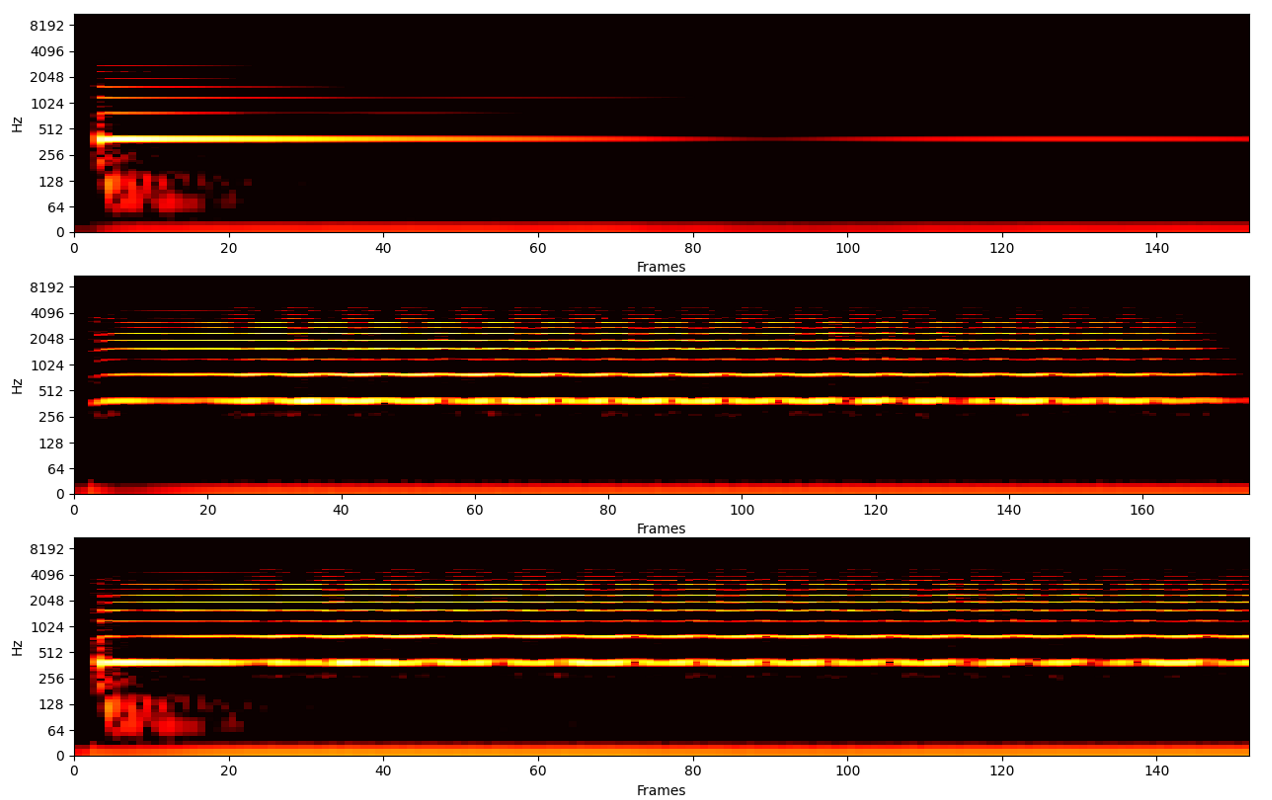
\includegraphics[width=\linewidth]{ch2/fig-G4-violin-piano.png}
    \caption{小提琴與鋼琴演奏G4音高三秒的特徵圖\ 上:小提琴,中:鋼琴,下:混合}
    \label{fig:fig-ch2-G4-violin-piano}
\end{figure}

雖然人耳可以輕易分辨出不同的音色,
但是當兩種聲音混合在一起時,要精準的將兩種樂器的聲音分開是一件困難的任務,
\cref{fig:fig-ch2-G4-violin-piano}的下方圖顯示了音訊混合後的特徵長相,
若要將兩種樂器的音源分離,我們必須精準地知道每個頻率原本的成分才有可能乾淨的分離。
音源分離的難度與樂器音色的複雜度、樂器種類的相似度而提高,因此至今音源分離的任務還是非常具有挑戰性。

另外在音樂追蹤方面,使用兩段相似的音訊特徵來追蹤是常見的方法,特徵越相近越容易有好的追蹤結果,
但若是屬於音色變化較大的樂器(例如小提琴),儘管是同一人演奏相同曲目兩次,特徵也不一定相同,
\cref{fig:fig-ch2-beethoven-violin-play-twice}顯示同一人使用相同速度、曲目演奏兩次的特徵圖,
雖然大致上看起來都相同,但細看的話在時間軸為100 frames時,兩邊的特徵還是有些微的不同,
這些些微的不同之處都有可能會影響到追蹤結果。
\cref{fig:fig-ch2-bwv1006-two-different-violin}顯示不同人演奏同一首曲子的特徵圖,
可以看到這兩段音訊明顯在環境的收音上可能差很多,且在曲子的詮釋上也不完全相同,
使用這兩段音訊來追蹤,難度會比同一人演奏的情況要高很多,
因此使用不同音訊特徵來追蹤是具有一定的挑戰性。

\begin{figure}[H]
    \centering
    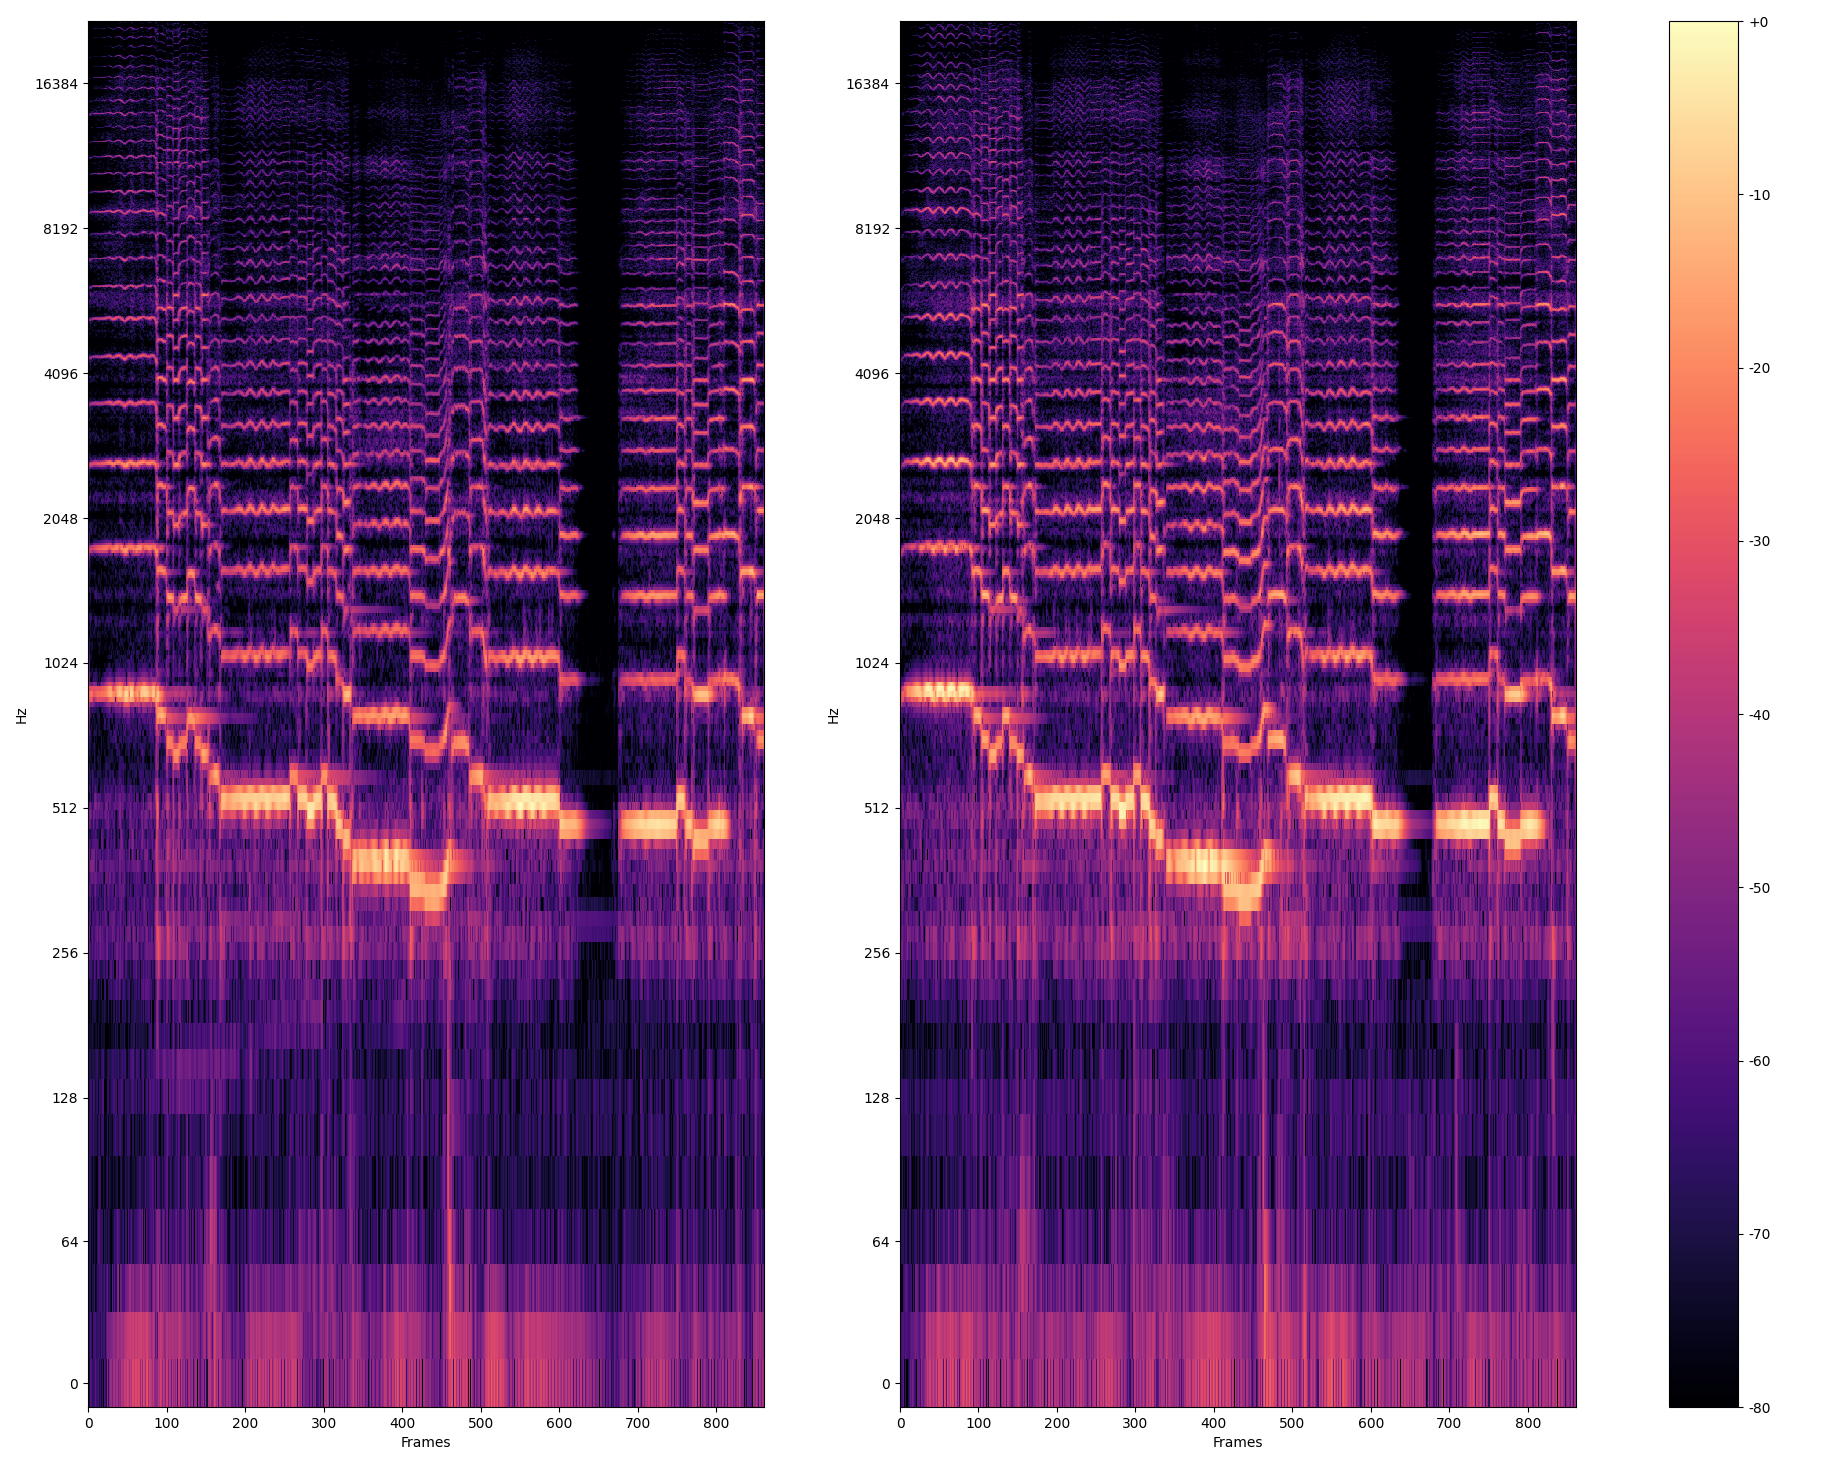
\includegraphics[width=1.0\linewidth, height=0.6\linewidth]{ch2/fig-beethoven-violin-play-twice.png}
    \caption{同一人演奏兩次 Beethoven Spring Sonata No.1 之特徵圖}
    \label{fig:fig-ch2-beethoven-violin-play-twice}
\end{figure}

\begin{figure}[H]
    \centering
    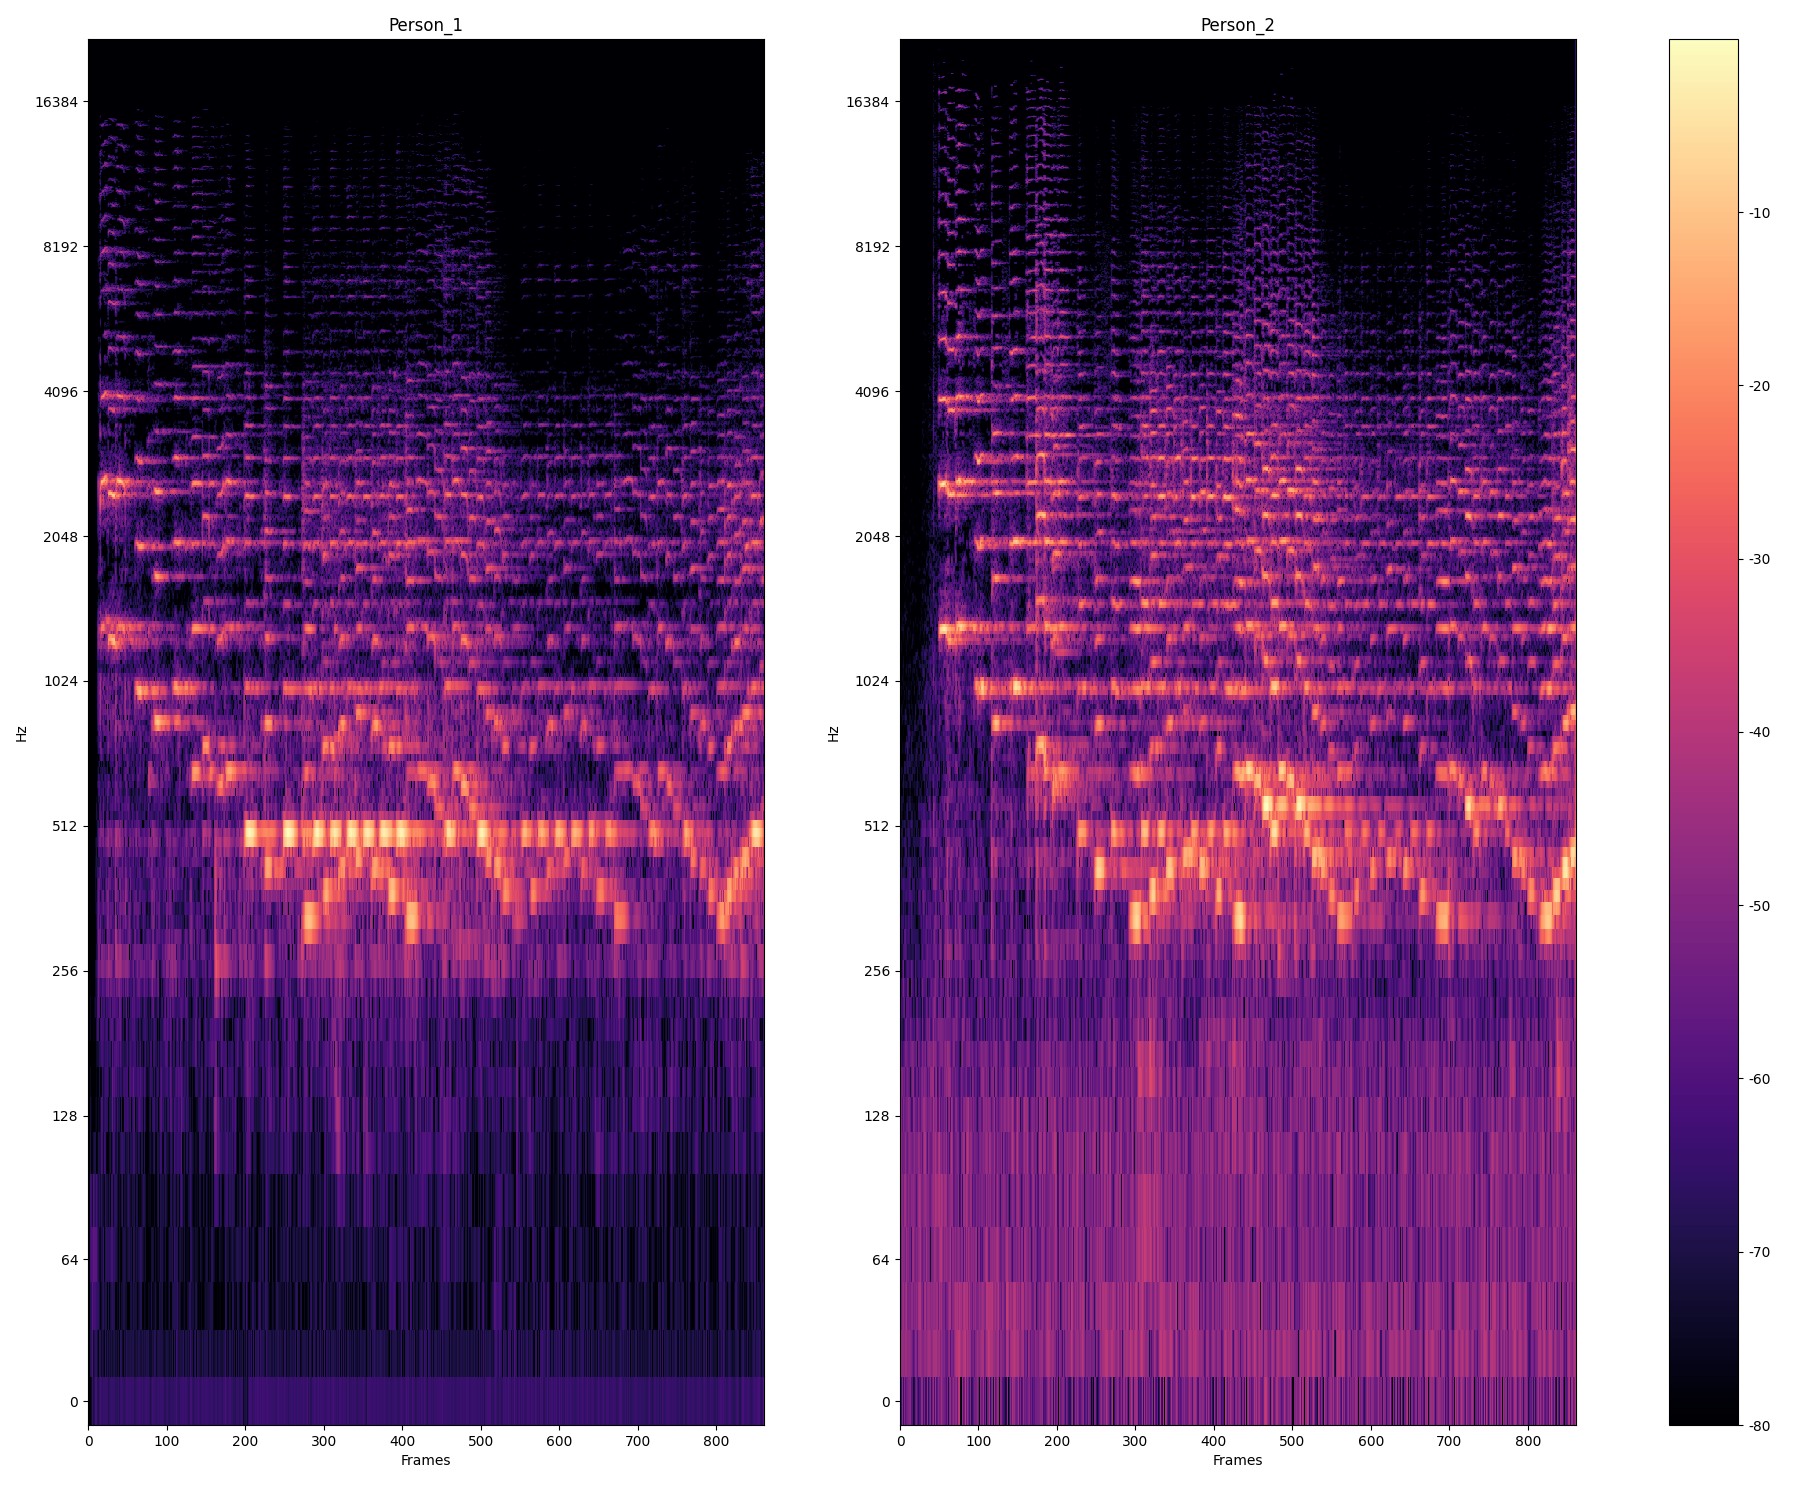
\includegraphics[width=1.0\linewidth, height=0.6\linewidth]{ch2/fig-bwv1006-two-different-violin.png}
    \caption{不同人演奏 Bach BWV1006 之特徵圖}
    \label{fig:fig-ch2-bwv1006-two-different-violin}
\end{figure}

\pagebreak

\section{文獻回顧}
\subsection{音源分離相關研究}
音源分離為MIR中的一個重要領域,日常生活中我們所聽到的音樂大多數是來自多個音源的混合音訊,
許多人可能希望調整混合音訊中的某種樂器的聲音平衡、改變聲音的空間位置,
甚至將混合音訊與每個存在於其中的音樂來源作為其他MIR任務的訓練資料,
因此,若是可以取得每個音樂來源的單獨音訊,上述所說的應用都能夠實現。

音源分離的目標最常見的為分離一首包含人聲、貝斯、鼓與其他(非前三者的所有音訊)的歌曲,
在大型音源分離比賽~\cite{Yuki_Mitsufuji2021MusicDemixing, Fabbro_Giorgio2023TheSoundDemixing}
中也是使用此標準進行。音源分離的方法可分為基於時間頻率表示方法與基於波形表示方法,
第一種通常會預測每個來源的功率頻譜,並結合輸入的混合音訊相位來合成每個音源的波形,
較傳統的方法有獨立成分分析(Independent Components Analysis, ICA)~\cite{comon1994independent},
此方法的目標是找到一個分離矩陣,使混合訊號透過分離矩陣計算出獨立的來源訊號;
非負矩陣分解(Non-negative Matrix Factorization, NMF)~\cite{lee2000algorithms}
為一種非監督式的機器學習技術,此方法是希望找到最好的兩個矩陣,使他們的乘積能接近原始的輸入。
然而這兩種方法對於複雜的混合音訊通常無法完全恢復單個音訊。
近年來隨著深度學習領域的蓬勃發展,
越來越多研究使用全連接神經網路(Fully-Connected Neural Network, FC)、
長短期記憶模型(Long Short-Term Memory, LSTM)、
遞歸神經網路(Recurrent Neural Networks, RNN)等方法訓練頻譜圖。
2018年由Stöter等人所提出的Open-Unmix~\cite{FabianRobert_Stöter2019OpenUnmix}
模型在當時在公開資料集MUSDB~\cite{Rafii2017musdb18}上表現最佳,
此模型使用三層雙向LSTM對輸入預測一個遮罩,將混合音訊透過遮罩得到分離音源頻譜圖。
隨後在2022年由Luo Yi等人所提出的Band-Split RNN~\cite{Luo_Yi2022MusicSourceSeparation}
在MUSDB上取得最佳的成績,此模型將輸入的頻譜圖分割為預先定義好頻帶寬度的子帶頻譜圖,
將子帶頻譜圖轉為相同維度的特徵後利用堆疊RNN交錯訓練,
最後經過多層感知機(Multilayer Perceptron, MLP)
生成遮罩並與混合輸入結合產生分離音源頻譜圖,
至今仍是基於時間頻率訓練的開源模型中效果最佳的模型。
Open-Unmix與Band-Split RNN皆允許使用者自訂不同的分離目標,
使的這兩個模型擁有很高的靈活性。

第二種基於波形訓練的方法最早提出的模型為Wave-U-Net~\cite{stoller2018wave},
近年來較多人使用的Demucs~\cite{défossez2021music}就是基於Wave-U-Net的架構開發的,
Demucs為Encoder/Decoder架構,內部由卷積Encoder/Decoder與雙向LSTM組成,
Encoder與Decoder使用Skip U-net連接,將混合立體音訊作為輸入,輸出每個來源的估計波型。
2021年MDX競賽~\cite{Yuki_Mitsufuji2021MusicDemixing}
由Meta AI提出的冠軍模型Hybrid Demucs~\cite{defossez2021hybrid}更是將Demucs擴展為多域分析的架構,
模型變為由波型、頻譜和共享層組成。2022年Meta AI結合先前的結果提出了
Hybrid Transformers~\cite{rouard2023hybrid},將Encoder/Decoder內部兩層替換為跨域Transformer,
使的模型可以接受異質資料,變成更靈活的架構,2023年在MUSDB上取得最佳的成績,
為目前所有開源模型中最佳的模型。

在古典樂器錄音的音源分離研究中,
由於大部分混合音訊中的樂器皆為音高樂器(例如:鋼琴、小提琴等等),
比起音高樂器與非音高樂器(例如:鼓)的音源分離情況更有挑戰性,
且公開資料集的蒐集難度高,導致訓練模型的難度也更大。
因此針對這些資料通常會使用資料增強的方法來增加訓練資料,
由Miron等人提出的CNN-based低延遲單聲道源分離模型~\cite{miron2017generating},
透過改變速度、音色、動態時間局部變化來增加新的訓練資料,使模型在實際情況下更能應對演奏時的狀況。
由Chiu Ching Yu等人提出針對資料規模小的資料集的資料增強方法~\cite{Chiu_ChingYu2020MixingSpecific},
使用Open-Unmix模型作為架構提出Aug4mss模型,並在針對小提琴與鋼琴的混合音源分離的任務上,
比當時可用的最佳模型Spleeter~\cite{hennequin2020spleeter}的效果要好。

本研究將使用靈活性高且較輕量的Band-Split RNN~\cite{Luo_Yi2022MusicSourceSeparation}模型,
針對小提琴與鋼琴的混合音源資料做訓練,旨在促進古典樂器錄音的音源分離研究進展。

% 引用音源分離的相關論文並進一步討論

\subsection{音樂追蹤相關研究}
音樂追蹤在MIR領域中是一項重要的應用,與節拍追蹤~\cite{heydari2021don, goto2021musical, di2021downbeat}、
樂譜追蹤~\cite{henkel2019score}、自動伴奏~\cite{zhang2023design}等相關技術有密切的關係,
本節專注探討以音訊特徵為主的即時音樂追蹤方法與應用的相關研究。

音樂追蹤的方法包含隱藏馬爾科夫模型(Hidden Markov Model, HMM)~\cite{cano1999score},
HMM透過特徵觀察每個狀態的機率迭帶訓練更新目前追蹤的位置,但由於HMM依賴於離散空間來表示樂譜的音符與節奏,
因此不適合處理複雜的連續變化,且因為計算複雜性高,在即時表現方面較為遜色;
動態時間規整(Dynamic Time Warping, DTW)~\cite{Arzt2012Adaptive, Raffel2016Optimizing}為最多人使用的方法之一,
DTW透過計算兩段相似序列的成本矩陣,回推兩段音訊的最佳對齊點,
由於音樂的連續性使的DTW計算結果準確率高,
但也因為計算時間複雜度高而無法應用在即時的音樂追蹤。
因此許多人對DTW演算法改良了更快速的版本,
例如平行化動態時間規整(Parallel Dynamic Time Warping, PDTW)~\cite{Wei2018Online},
PDTW將兩個時間序列分割成多段的序列,每段序列各自計算DTW,計算完畢後再將每段序列連接回整段,
加速DTW的運算時間;
線上動態時間規整(Online Dynamic Time Warping, ODTW)~\cite{dixon2005ODTW, Arzt2010Towards, Lin2020AHumanComputerDuetSystem}
將原本DTW向後對齊的模式改為增量對齊,並限制了的搜索範圍,
ODTW不需要事先取得兩段序列的資訊,
而是根據每個時間點計算出的路徑決定下一步的方向,
因此ODTW在即時音訊的處理的情況會比前面提到的方法還要快速,
更能達到即時音樂追蹤的效果,但也因為無法確定哪個位置為音訊結束的位置,
,因此通常追蹤的準確率會比DTW要低。

音訊特徵的音樂追蹤比起使用MIDI檔案的音樂追蹤要困難許多,
因為追蹤結果對特徵的變化非常敏感,因此使用的音訊特徵通常越相像越好,
例如使用同一人事先演奏的音訊來追蹤同一人的現場演奏,
但通常使用者並不會特意去錄製事先演奏的音訊,尤其是在沒有合奏者的情況下,
因此本研究致力於研究使用不同音訊特徵來追蹤現場演奏的即時音樂追蹤系統。
本研究將基於~\cite{Lin2020AHumanComputerDuetSystem}所提出的架構進行重新實現
並針對ODTW演算法與部分方法進行改動,希望能藉此達到我們所期望的效果並促進即時音樂追蹤研究進展。

% DTW、DTW的各種變形、ODTW、RL、
% 引用音樂追蹤的相關論文並進一步討論

\pagebreak

\end{document}